%\documentclass[11pt,a4paper]{report}
\documentclass{article}
\usepackage[top=1in, bottom=1in, left=1in, right=1in]{geometry}

%%%%%%%%%%%%%%%%
%%% PACKAGES %%%
%%%%%%%%%%%%%%%%

\usepackage{amsmath}
\usepackage{graphicx}
\usepackage{parskip}

% used with figures:
\usepackage{float}
\usepackage{caption}
\usepackage{subcaption}

\graphicspath{{./img/}}


%%%%%%%%%%%%%
%%% INFOS %%%
%%%%%%%%%%%%%

\title{computer gestuurde regeltechnieken - Part I}
\author{Willem Melis (r0348639)}
\date{\today}

\setcounter{MaxMatrixCols}{20}

%%%%%%%%%%%%%%%%
%%% DOCUMENT %%%
%%%%%%%%%%%%%%%%

\begin{document}

\begin{titlepage}
\begin{center}


\includegraphics[width=3cm]{kuleuven.jpg}~\\[1cm]
\vfill


\textsc{\LARGE KU Leuven}\\[0.7cm]

\textsc{\Large Computer gestuurde regeltechnieken}\\[0.7cm]
\textsc{\Large Exercises - Part 1 }\\[0.7cm]



\centering \huge \bfseries Case study: Quadcopter

\end{center}

\vfill

% auteurs et tuteur
\begin{center}
\emph{Author:} \\[.2cm]
\begin{tabular}[h]{rl}
Willem \textsc{Melis} & r0348639\\
\phantom{------------------------} & \phantom{------------------------}\\
\end{tabular}
\end{center}

\vfill

\begin{center}
\begin{tabular}[h]{rl}
\emph{Professor:} & Bart \textsc{De Moor} \\
\emph{Assistants:}&  
Oscar Mauricio  \textsc{Agudelo} \\
&  Supinya  \textsc{Piampongsant} \\
\phantom{------------------------} & \phantom{------------------------}\\
\end{tabular}
\end{center}

\vfill
\vfill
\vfill

%date
\begin{center} 
2016 - 2017 \\[.5cm]
{\Large \today}
\end{center}

\end{titlepage}

\tableofcontents 
\newpage

\section{Introduction}
The report tries to follow the order of the assignment as much as possible. For each part there is Matlab code, the appendix briefly explains which files belong to which part of the report. Some of the figures are added as an appendix. The text specifically refers to them when the reader should take a look at them, they are of little value on there own.
\section{Linearizion}

\subsection{Find equilibrium point}

Find the fix point with $$x=y=z=\phi=\theta=\psi=0$$

If the system is filled out with these parameters a much simpler set of equations is obtained:

\begin{eqnarray}
\dot{x}=v_x \\
\dot{y}=v_y \\
\dot{z}=v_z \\
\dot{v_x}=-\frac{k \ d}{m}v_x \\
\dot{v_y}=-\frac{k \ d}{m}v_y \\
\dot{v_z}=-\frac{k \ d}{m}v_z -g + \frac{K \ C_m}{m}(v_1^2+v_2^2+v_4^2+v_4^2)\\
\dot{\phi}=w_x \\
\dot{\theta}=w_y \\
\dot{\psi}=w_z \\
\dot{w_x}=\frac{L \cdot k \cdot C_m}{I_{xx}}(v_1^2 - v_3^2) - \frac{I_{yy}-I_{zz}}{I_{xx}} w_y  w_z \\
\dot{w_y}=\frac{L \cdot k \cdot C_m}{I_{xx}}(v_2^2 - v_4^2) - \frac{I_{zz}-I_{xx}}{I_{yy}} w_y  w_z\\
\dot{w_z}=\frac{b \cdot C_m}{I_{yy}}(v_1^2-v_2^2+v_3^2-v_4^2) - \frac{I_{xx}-I_{yy}}{I_{zz}}w_y  w_z
\end{eqnarray}

Its very clear from the that $v_x,v_y,x_z,w_x,w_y$ and $w_z$ are zero ,the remaining equations are set equal to zero :

\begin{eqnarray}
\dot{v_z}= -g + \frac{K \ C_m}{m}(v_1^2+v_2^2+v_4^2+v_4^2) =0\\
\dot{w_x}=\frac{L \cdot k \cdot C_m}{I_{xx}}(v_1^2 - v_3^2) =0 \\
\dot{w_y}=\frac{L \cdot k \cdot C_m}{I_{xx}}(v_2^2 - v_4^2) =0\\
\dot{w_z}=\frac{b \cdot C_m}{I_{yy}}(v_1^2-v_2^2+v_3^2-v_4^2) =0
\end{eqnarray}

simplify even further:

\begin{eqnarray}
g =  \frac{K \ C_m}{m}(v_1^2+v_2^2+v_4^2+v_4^2)\\
v_1^2 - v_3^2 =0 \\
v_2^2 - v_4^2 =0\\
v_1^2-v_2^2+v_3^2-v_4^2 =0
\end{eqnarray}

This means that
\begin{eqnarray}
v_1^2 = v_3^2 \\
v_2^2 = v_4^2 \\
\end{eqnarray}

combine this with the last equation:

\begin{equation}
v_1^2=v_2^2=v_3^2=v_4^2
\end{equation}

This is to be expected as the motors should all be running at the same speed to Hoover. The speed at which these motors need to rotate depends on the gravity which is the last equation $$g =  \frac{K \ C_m}{m}(v_1^2+v_2^2+v_4^2+v_4^2) \\$$ As all the voltages are exactly the same this becomes: $$\frac{m \cdot g}{K \cdot C_m \cdot 4}=   v_i^2 = u_i \\$$ with $i=1...4$

and: $$v_1^2+v_2^2+v_3^2+v_4^2=\frac{m \cdot g}{K \cdot C_m}$$ 

\subsection{Define linear model}

The lineare model is of the form $$\triangle \dot{x}=A\triangle x + B\triangle u $$ $$ \triangle y=C\triangle x$$

The matrix is the Jacobian related to x and matrix B is the Jacobian related to u both evaluated in the equilibrium point.

$$x=[x \ y \ z \ v_x \ v_y \ v_z \ \phi \ \theta \ \psi w_x w_y w_z]  $$
$$x_{equilibrium} = [0\ 0\ 0\ 0\ 0\ 0\ 0\ 0\ 0\ 0\ 0\ 0]$$

$$
u_{equilibrium} =
 [\frac{m \cdot g}{K \cdot C_m \cdot 4} \frac{m \cdot g}{K \cdot C_m \cdot 4} \frac{m \cdot g}{K \cdot C_m \cdot 4} \frac{m \cdot g}{K \cdot C_m \cdot 4}] 
$$

$$
A(x_{equilibrium}) =
\begin{bmatrix}
0 & 0 & 0 & 1 & 0 & 0 & 0 & 0 & 0 & 0 & 0 & 0 \\
0 & 0 & 0 & 0 & 1 & 0 & 0 & 0 & 0 & 0 & 0 & 0 \\
0 & 0 & 0 & 0 & 0 & 1 & 0 & 0 & 0 & 0 & 0 & 0 \\

0 & 0 & 0 & -\frac{k_d}{m} & 0 & 0 & 0 & g & 0 & 0 & 0 & 0 \\
0 & 0 & 0 & 0 & -\frac{k_d}{m} & 0 & -g & 0 & 0 & 0 & 0 & 0 \\
0 & 0 & 0 & 0 & 0 & -\frac{k_d}{m} & 0 & 0 & 0 & 0 & 0 & 0 \\

0 & 0 & 0 & 0 & 0 & 0 & 0 & 0 & 0 & 1 & 0 & 0 \\
0 & 0 & 0 & 0 & 0 & 0 & 0 & 0 & 0 & 0 & 1 & 0 \\
0 & 0 & 0 & 0 & 0 & 0 & 0 & 0 & 0 & 0 & 0 & 1 \\

0 & 0 & 0 & 0 & 0 & 0 & 0 & 0 & 0 & 0 & 0 & 0 \\
0 & 0 & 0 & 0 & 0 & 0 & 0 & 0 & 0 & 0 & 0 & 0 \\
0 & 0 & 0 & 0 & 0 & 0 & 0 & 0 & 0 & 0 & 0 & 0
\end{bmatrix}
$$



$$
u = [u_1 \ u_2 \ u_3 \ u_4] = [v_1^2 \ v_2^2 \ v_3^2 \ v_4^2 ]
$$

$$
B(u_{equilibrium}) = 
\begin{bmatrix}
0 & 0 & 0 & 0 \\ %x
0 & 0 & 0 & 0 \\ %y
0 & 0 & 0 & 0 \\ %z

0 & 0 & 0 & 0 \\ %vx dot
0 & 0 & 0 & 0 \\ %vy dot
\frac{k c_m}{m} & \frac{k c_m}{m} & \frac{k c_m}{m} & \frac{k c_m}{m} \\

0 & 0 & 0 & 0 \\
0 & 0 & 0 & 0 \\
0 & 0 & 0 & 0 \\

\frac{L K c_m }{I_{xx}} & 0 & -\frac{L K c_m }{I_{xx}} & 0 \\
0 & \frac{L K c_m }{I_{yy}} & 0 & -\frac{L K c_m }{I_{yy}} \\
\frac{b c_m }{I_{zz}} & -\frac{b c_m }{I_{zz}} & \frac{b c_m }{I_{zz}} & -\frac{b c_m }{I_{zz}}\\
\end{bmatrix}
$$


\section{discretization}
\subsection{options}
The 3 options are zero-order hold, Euler's rule and the bilinear transformation. (using a sampling time of $T_s=0.05s$). The matrix A is not invertible which means that the zero and hold is not viable. 

\subsection{choice discretization rule}
The bilinear transformation always maps stable poles in the continuous domain to stable poles in the discrete domain. However in this particular case both Euler and the bilinear transformation have stable poles. The are both fully controllable and observable. The only real difference is in the transmission zeros, the  bilinear transformation has transmission zeros while Euler does not. This makes the  bilinear transformation the preferred choice in this case. As transmission zeros are stable which means the system is minimum phase system as the 8 transmission zeros are all -1 which is inside the unit circle.

\section{LQR controller without payload}
\subsection{full-state feedback controller}

The controller is constructed in Simulink (Figure~\ref{fig:simulink diagram full-state feedback controller}) according to the diagram on page 221 of the course notes. A type 1 full-state feedback was used as its more robust, which is desirable as its controlling a flying object. 

\begin{figure}[H]
	\centering
	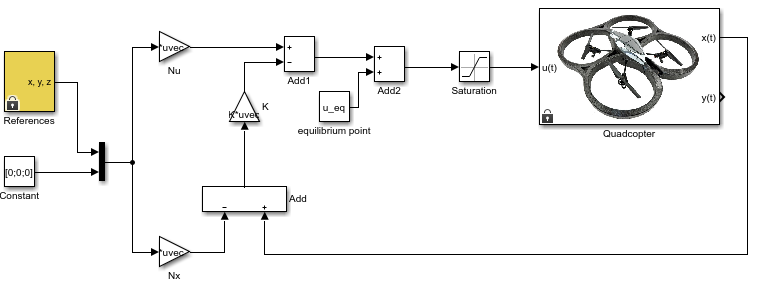
\includegraphics[width=0.5\textwidth]{./LQR_noload/full_state_feedback_simu.png}
	\caption{simulink diagram full-state feedback controller}
	\label{fig:simulink diagram full-state feedback controller}
\end{figure}

The matrix K is calculate with the LQR method as we did in the second exercise session. However in order to do LQR we need a matrix Q and R. As LQR minimizes $J_N = \frac{1}{2} \sum_{k=0}^{N-1}[x_k^TQx_k + u^T_kRu_k] + \frac{1}{2}x_N^TQx_N$. Notice how Q determines the weights given to $x_k$ and and R determines the weights given to $u_k$. 

If Q and R are taken as an diagonal matrix with ones on the diagonal then the quad copter does not have enough power to stay in the air. This is displayed in Figure~\ref{fig:full-state controller with simple diagonal matrices as Q and R}. Its very clear from Figure~\ref{fig:full-state controller with simple diagonal matrices as Q and R demo bad z position} that the controller does not optimize enough on the z axis.

\begin{figure}[H]
	\centering
	\begin{subfigure}[b]{0.3\textwidth}
		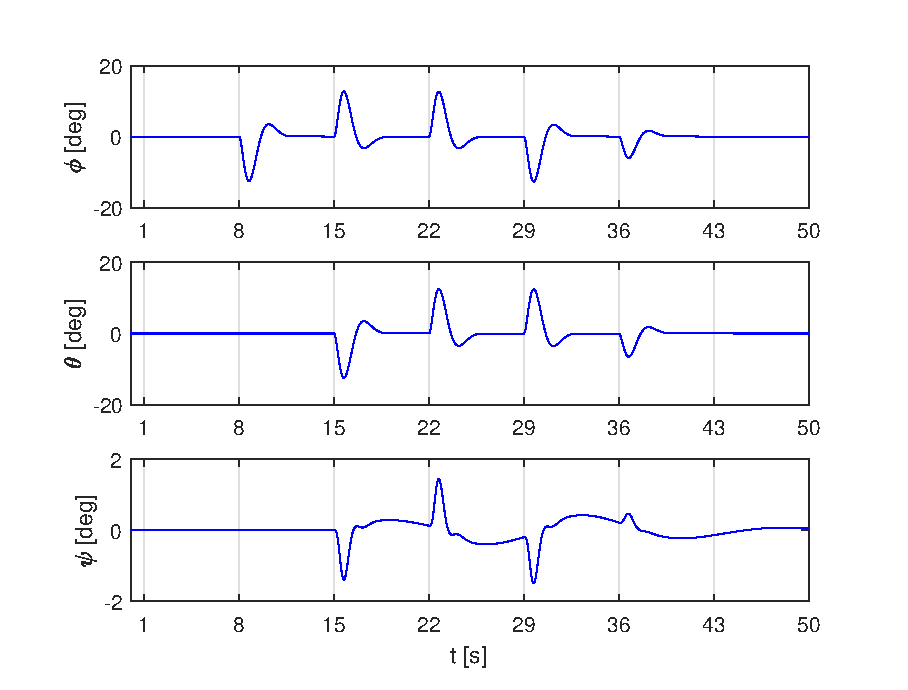
\includegraphics[width=\textwidth]{./LQR_noLoad/full_state/full_state_feedback_first_fig4.eps}
		\caption{angles}
	\end{subfigure}
	\begin{subfigure}[b]{0.3\textwidth}
		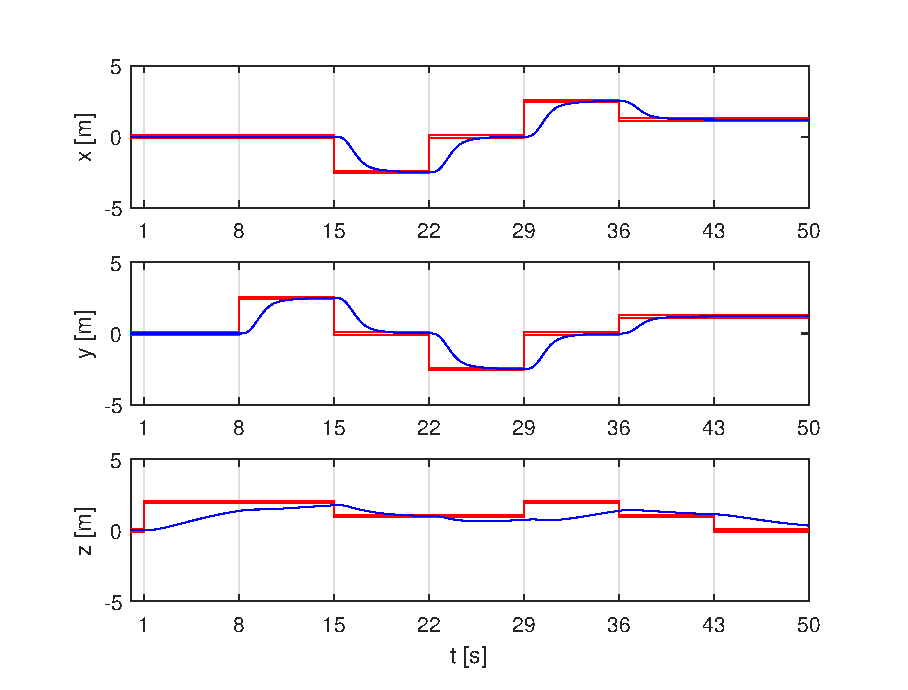
\includegraphics[width=\textwidth]{./LQR_noLoad/full_state/full_state_feedback_first_fig3.eps}
		\caption{position}
		\label{fig:full-state controller with simple diagonal matrices as Q and R demo bad z position}
	\end{subfigure}
	\begin{subfigure}[b]{0.3\textwidth}
		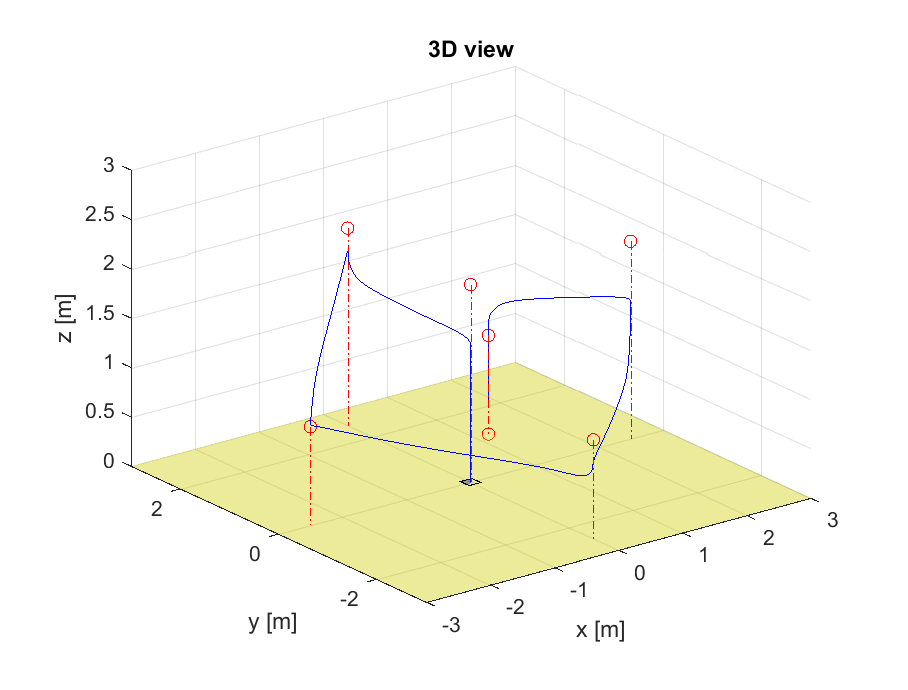
\includegraphics[width=\textwidth]{./LQR_noLoad/full_state/full_state_feedback_first_fig2.eps}
		\caption{track}
	\end{subfigure}
	\caption{full-state controller when Q and R are unit matrices}\label{fig:full-state controller with simple diagonal matrices as Q and R}
\end{figure}

In order to get a proper controller we need to put way more weight on the position z in the optimization problem. This is done by increasing a value in Q, as the z coordinate is an state. 

$$ 
Q=
\begin{bmatrix}
1 & 0 & 0 & 0 & ... \\
0 & 1 & 0 & 0 & ...\\
0 & 0 & 1 & 0 & ... \\
0 & 0 & 0 & 1 & ... \\
... & ... & ... & ... & ... 
\end{bmatrix}
=>
\begin{bmatrix}
1 & 0 & 0 & 0 & ... \\
0 & 1 & 0 & 0 & ...\\
0 & 0 & 10^2 & 0 & ... \\
0 & 0 & 0 & 1 & ... \\
... & ... & ... & ... & ... 
\end{bmatrix}
$$

\begin{figure}[H]
	\centering
	\begin{subfigure}[b]{0.3\textwidth}
		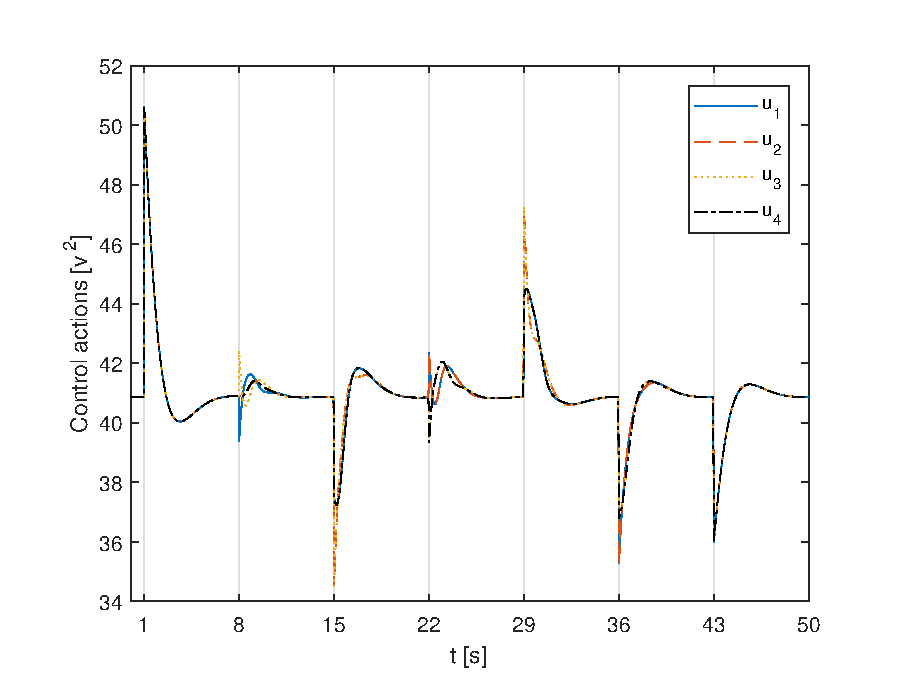
\includegraphics[width=\textwidth]{./LQR_noLoad/full_state/full_state_feedback_increased_z_fig5.eps}
		\caption{input voltages motors}
		\label{fig:full-state controller with low voltage}
	\end{subfigure}
	\begin{subfigure}[b]{0.3\textwidth}
		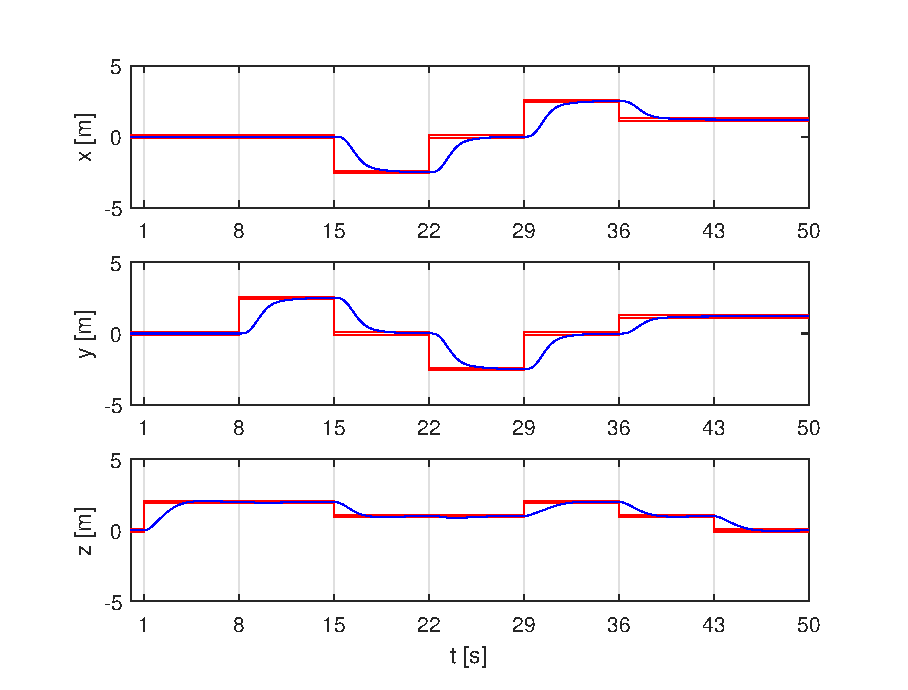
\includegraphics[width=\textwidth]{./LQR_noLoad/full_state/full_state_feedback_increased_z_fig3.eps}
		\caption{position on each axis}
	\end{subfigure}
	\begin{subfigure}[b]{0.3\textwidth}
		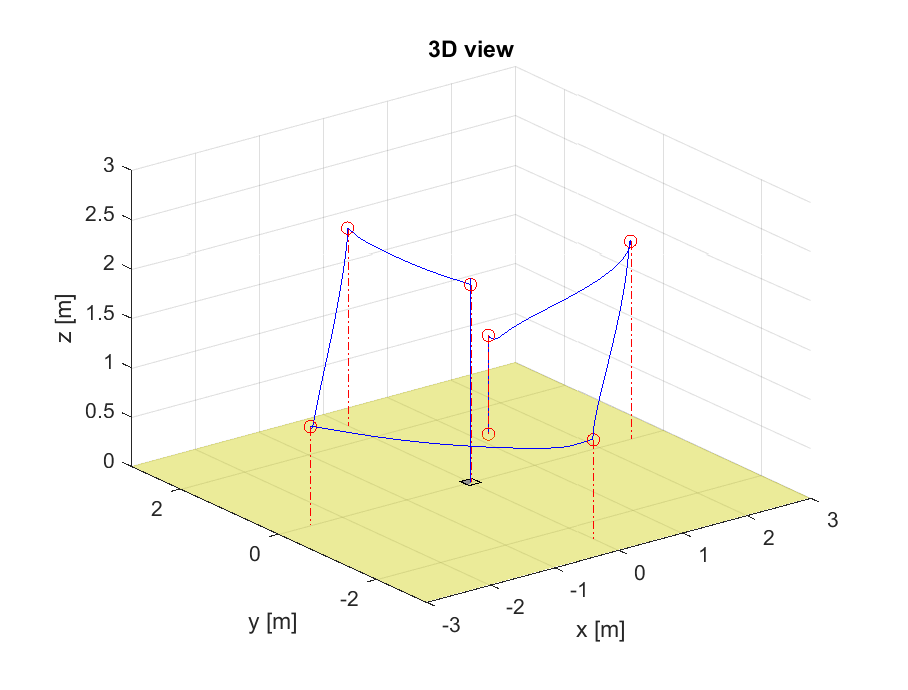
\includegraphics[width=\textwidth]{./LQR_noLoad/full_state/full_state_feedback_increased_z_fig2.eps}
		\caption{3D position}
	\end{subfigure}
	\caption{full-state controller with adjusted Q an unit matrix as R }\label{fig:full-state controller with adjusted Q matrix but a unit matrix as R}
\end{figure}

Figure~\ref{fig:full-state controller with adjusted Q matrix but a unit matrix as R} contains the results of the full state controller with the adjusted Q matrix. The quad-copter does reach all its checkpoint but the input voltages on the motors are rather low. 

Lowering the values of R  will result in higher voltages and so an increase speed. But keeping robustness in mind R must still be sufficiently large to avoid oscillating or extremely fast changes in voltages. A diagonal value of 0.1 seems to be reasonable for R, this is illustrated in Figure~\ref{fig:full-state controller with proper diagonal matrices as Q and R}.The adjustment of R improves the average time from 3.736 to 3.214 s. Notice how the voltage also get lower in Figure~\ref{fig:full-state controller with proper diagonal matrices as Q and R - voltages}, the controller is way more nervous then in Figure~\ref{fig:full-state controller with low voltage}.
\begin{figure}[H]
	\centering
	\begin{subfigure}[b]{0.3\textwidth}
		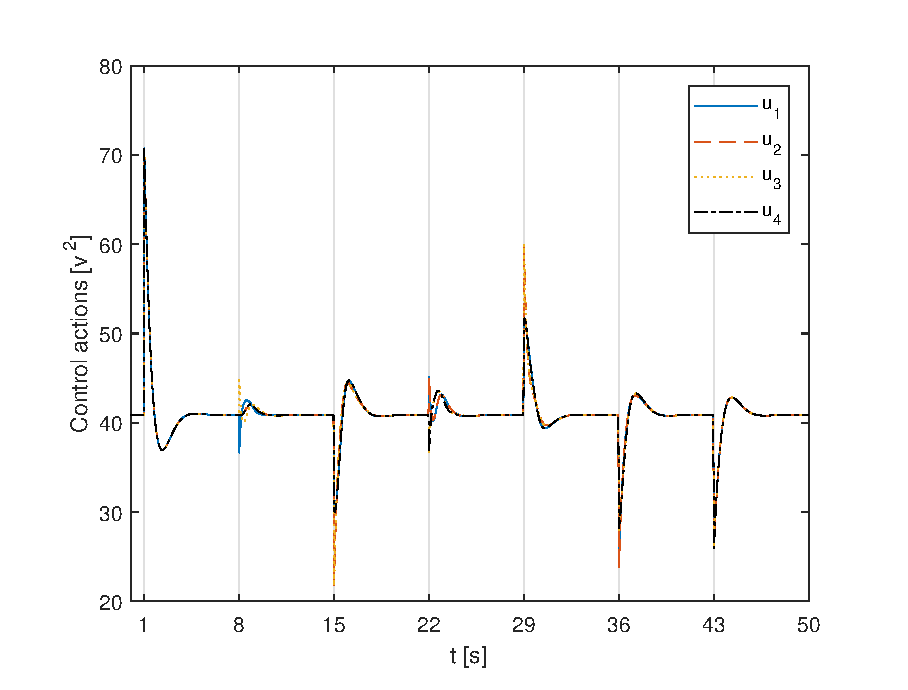
\includegraphics[width=\textwidth]{./LQR_noLoad/full_state/full_state_feedback_final_fig5.eps}
		\caption{angles}
		\label{fig:full-state controller with proper diagonal matrices as Q and R - voltages}
	\end{subfigure}
	\begin{subfigure}[b]{0.3\textwidth}
		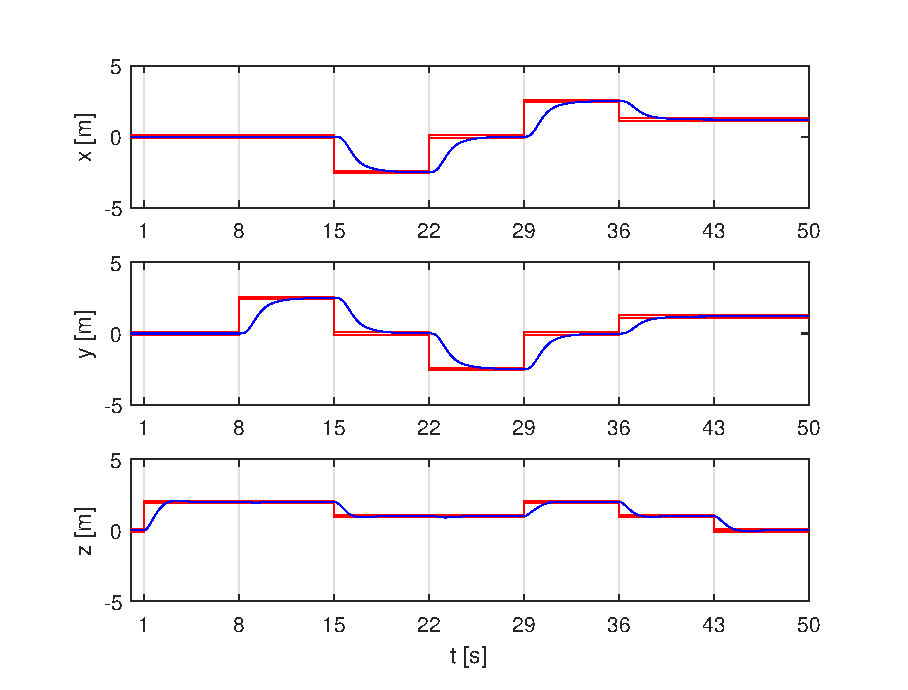
\includegraphics[width=\textwidth]{./LQR_noLoad/full_state/full_state_feedback_final_fig3.eps}
		\caption{position}
	\end{subfigure}
	\begin{subfigure}[b]{0.3\textwidth}
		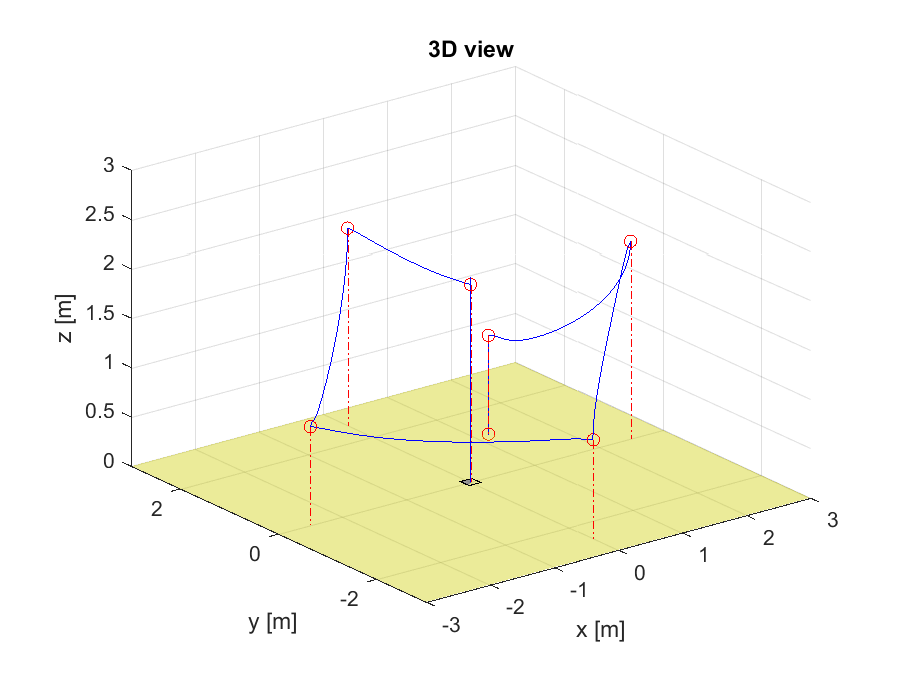
\includegraphics[width=\textwidth]{./LQR_noLoad/full_state/full_state_feedback_final_fig2.eps}
		\caption{track}
	\end{subfigure}
	\caption{full-state controller with proper diagonal matrices as Q and R}\label{fig:full-state controller with proper diagonal matrices as Q and R}
\end{figure}
\subsubsection{Final weight matrices}

$$
Q=\begin{bmatrix}
1 & 0 & 0 & 0 & 0 & 0 & 0 & 0 & 0 & 0 & 0 & 0 \\
0 & 1 & 0 & 0 & 0 & 0 & 0 & 0 & 0 & 0 & 0 & 0 \\
0 & 0 & 10^2 & 0 & 0 & 0 & 0 & 0 & 0 & 0 & 0 & 0 \\
0 & 0 & 0 & 1 & 0 & 0 & 0 & 0 & 0 & 0 & 0 & 0 \\
0 & 0 & 0 & 0 & 1 & 0 & 0 & 0 & 0 & 0 & 0 & 0 \\
0 & 0 & 0 & 0 & 0 & 1 & 0 & 0 & 0 & 0 & 0 & 0 \\
0 & 0 & 0 & 0 & 0 & 0 & 1 & 0 & 0 & 0 & 0 & 0 \\
0 & 0 & 0 & 0 & 0 & 0 & 0 & 1 & 0 & 0 & 0 & 0 \\
0 & 0 & 0 & 0 & 0 & 0 & 0 & 0 & 1 & 0 & 0 & 0  \\
0 & 0 & 0 & 0 & 0 & 0 & 0 & 0 & 0 & 1 & 0 & 0 & \\
0 & 0 & 0 & 0 & 0 & 0 & 0 & 0 & 0 & 0 & 1 & 0 & \\
0 & 0 & 0 & 0 & 0 & 0 & 0 & 0 & 0 & 0 & 0 & 1 & \\
0 & 0 & 0 & 0 & 0 & 0 & 0 & 0 & 0 & 0 & 0 & 0 & \\
0 & 0 & 0 & 0 & 0 & 0 & 0 & 0 & 0 & 0 & 0 & 0 & \\
0 & 0 & 0 & 0 & 0 & 0 & 0 & 0 & 0 & 0 & 0 & 0 & \\
\end{bmatrix}
$$
$$
R=\begin{bmatrix}
0.1 & 0 & 0 & 0 \\
0 & 0.1 & 0 & 0 \\
0 & 0 & 0.1 & 0 \\
0 & 0 & 0 & 0.1 \\
\end{bmatrix}
$$


\input{part4_integrator.tex}
\subsection{Comparison results}
The integrator is quiet fast with its 2.964 seconds run time compared to the 3.214 seconds run time of the full-state feedback controller. However the matrices Q and R where way harder to determine for the integrator then the full-state feedback controller. Even tough the integrator only hard 3 extra states, those states made it significantly harder to determine Q and R.


% Integrator 2.964 seconds
% LQR run time=3.214seconds

\section{With load}
\subsection{Full-state}
The full-state feedback controller seems to get into trouble when adding a weight of 0.1. Figure~\ref{fig: full state unadjusted , not strong enough } displays the path taken by the quad copter with load. The weight of 0.1 pushes the quad copter down on the z-axis, and the controller does not compensate enough. If the weight corresponding to z is increased from $10^2$ to $10^4$ the controller does however compensate enough.(see Figure~\ref{fig: full state , strong enough }, the average time is  2.929 s)
\begin{figure}[H]
	\centering
	\begin{subfigure}[b]{0.3\textwidth}
		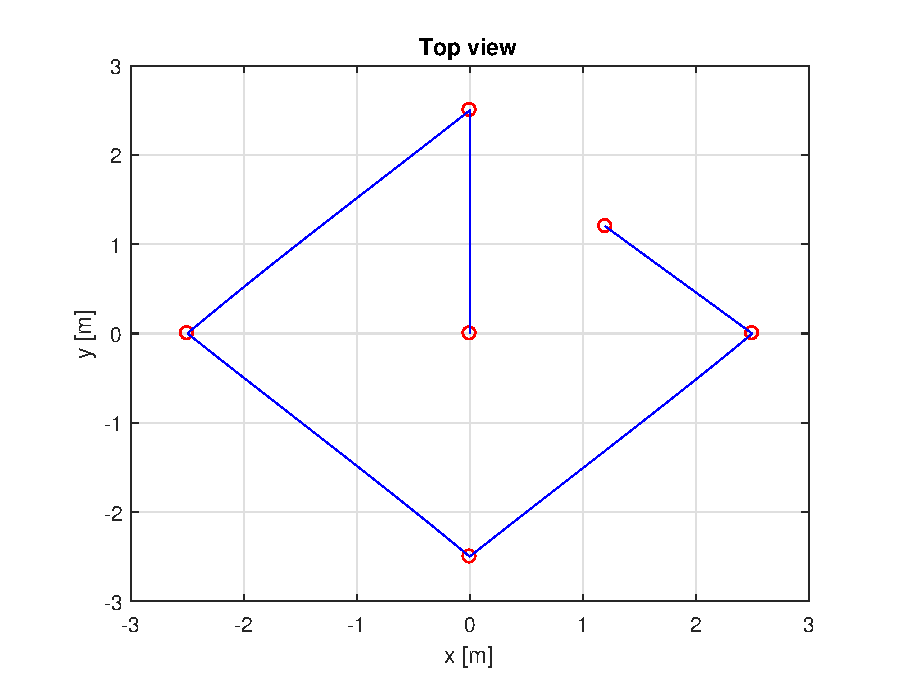
\includegraphics[width=\textwidth]{./LQR_load/fullState/noadjustment_fig1.eps}
		\caption{top view}
	\end{subfigure}
	\begin{subfigure}[b]{0.3\textwidth}
		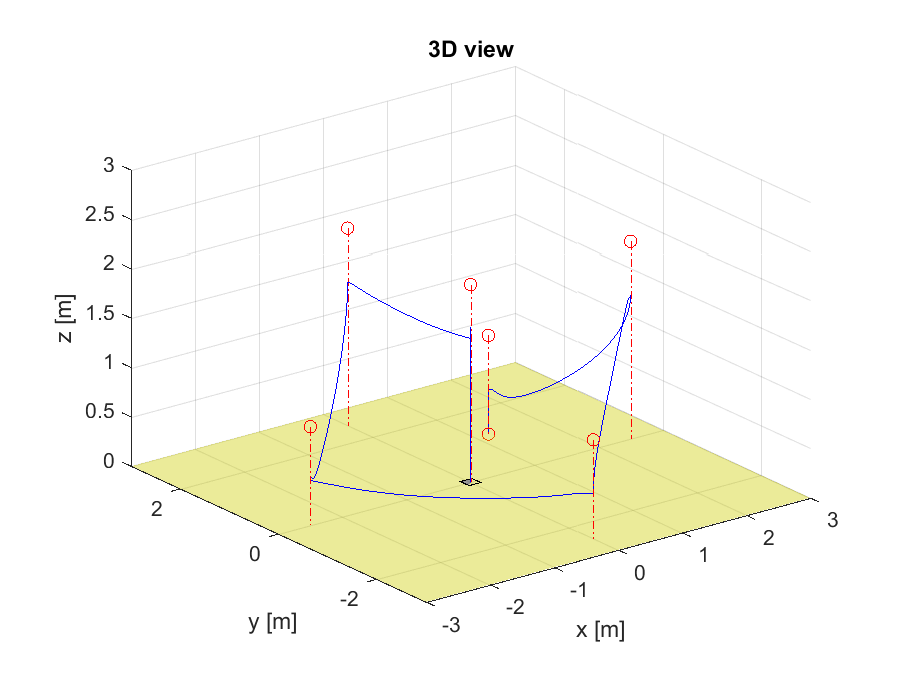
\includegraphics[width=\textwidth]{./LQR_load/fullState/noadjustment_fig2.eps}
		\caption{3D view}
		\label{fig: full state unadjusted , not strong enough }
	\end{subfigure}
	\begin{subfigure}[b]{0.3\textwidth}
		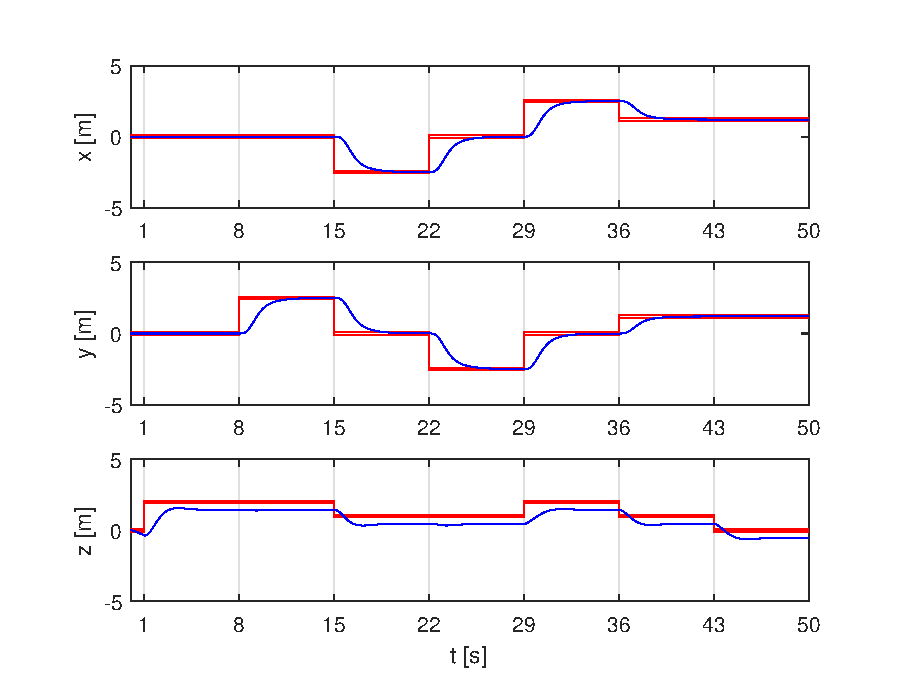
\includegraphics[width=\textwidth]{./LQR_load/fullState/noadjustment_fig3.eps}
		\caption{individual axis}
	\end{subfigure}
	\begin{subfigure}[b]{0.3\textwidth}
		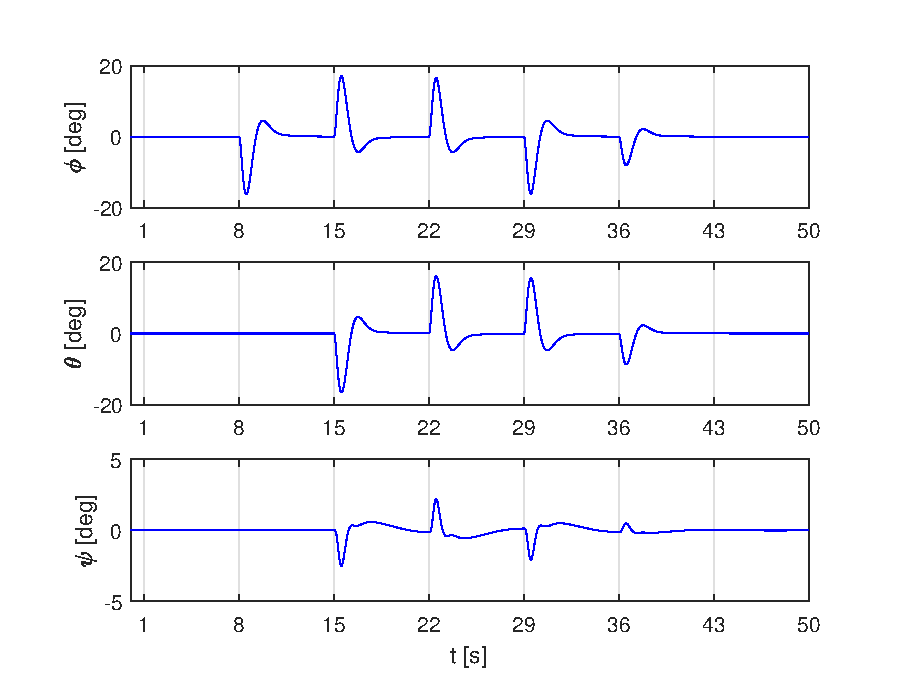
\includegraphics[width=\textwidth]{./LQR_load/fullState/noadjustment_fig4.eps}
		\caption{angles}
	\end{subfigure}
	\begin{subfigure}[b]{0.3\textwidth}
		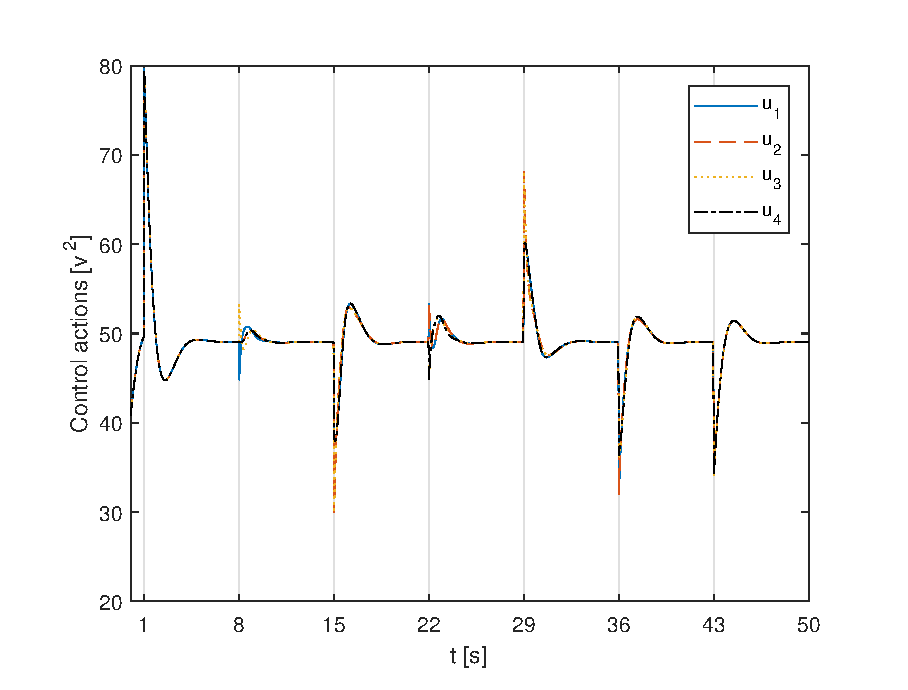
\includegraphics[width=\textwidth]{./LQR_load/fullState/noadjustment_fig5.eps}
		\caption{control actions}
	\end{subfigure}
	\caption{full state with 0.1 load, no adjustments to the weight matrices from the previous section }\label{fig:full state with load unadjusted}
\end{figure}

\begin{figure}[H]
	\centering
	\begin{subfigure}[b]{0.3\textwidth}
		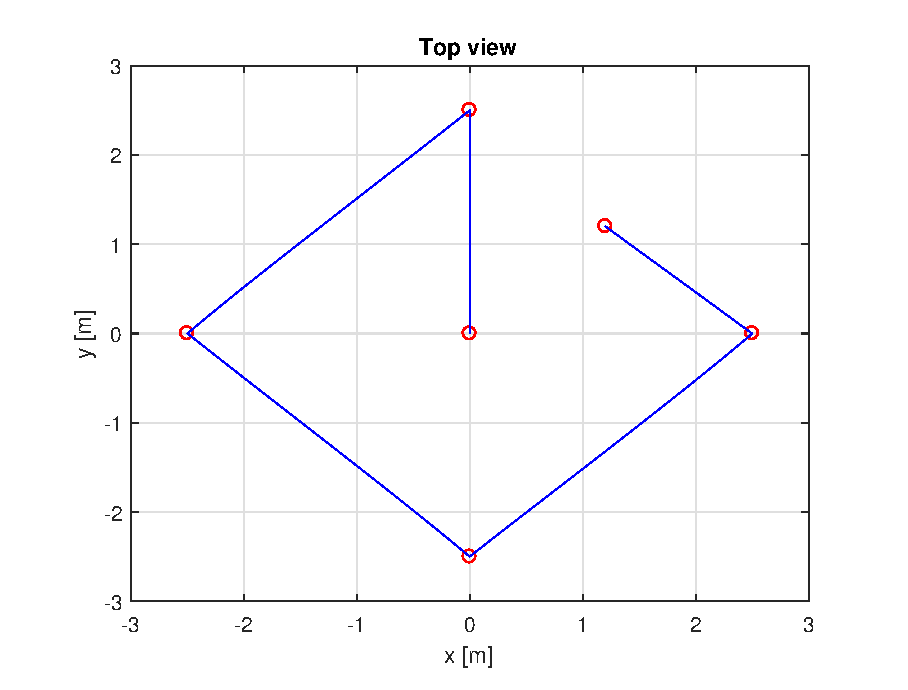
\includegraphics[width=\textwidth]{./LQR_load/fullState/fig1.eps}
		\caption{top view}
	\end{subfigure}
	\begin{subfigure}[b]{0.3\textwidth}
		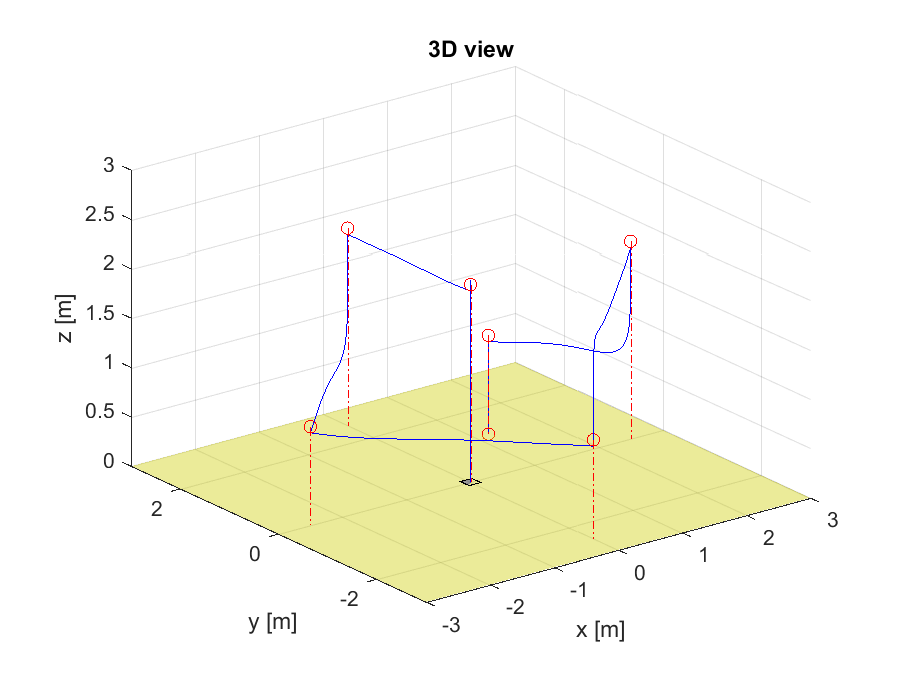
\includegraphics[width=\textwidth]{./LQR_load/fullState/fig2.eps}
		\caption{3D view}
		\label{fig: full state , strong enough }
	\end{subfigure}
	\begin{subfigure}[b]{0.3\textwidth}
		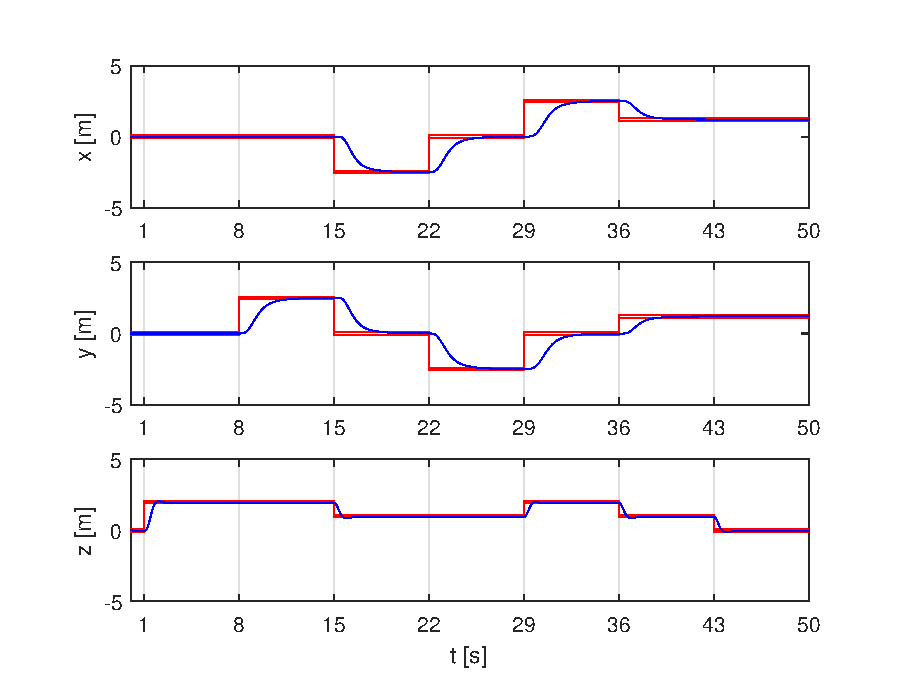
\includegraphics[width=\textwidth]{./LQR_load/fullState/fig3.eps}
		\caption{individual axis}
	\end{subfigure}
	\begin{subfigure}[b]{0.3\textwidth}
		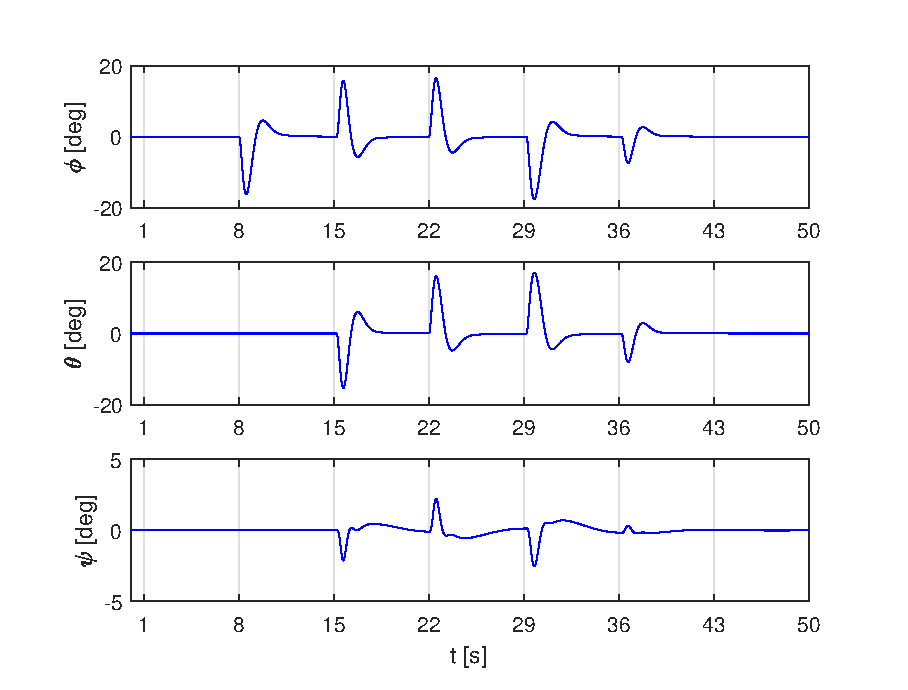
\includegraphics[width=\textwidth]{./LQR_load/fullState/fig4.eps}
		\caption{angles}
	\end{subfigure}
	\begin{subfigure}[b]{0.3\textwidth}
		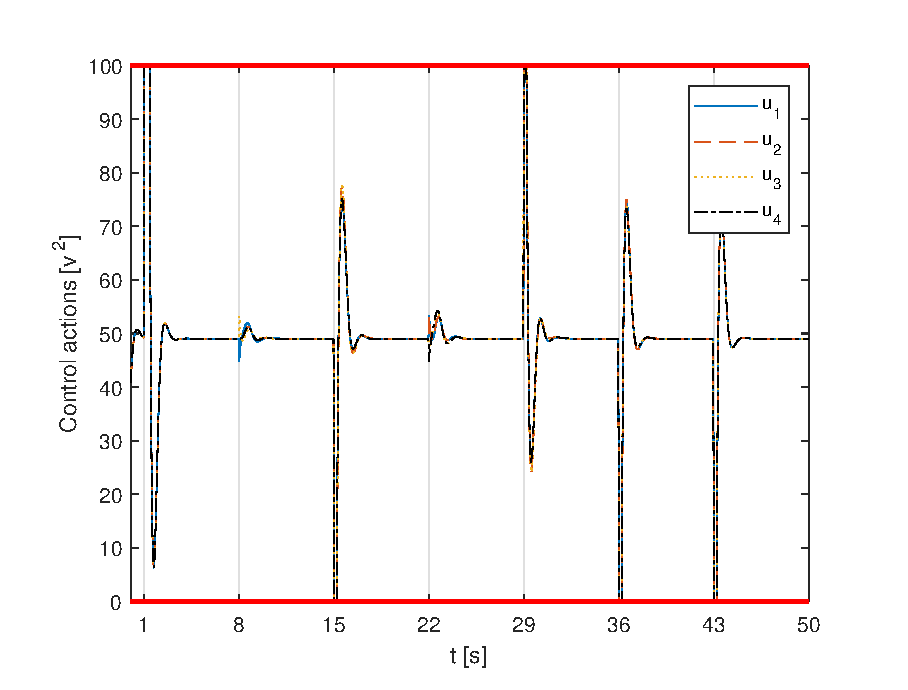
\includegraphics[width=\textwidth]{./LQR_load/fullState/fig5.eps}
		\caption{control actions}
	\end{subfigure}
	\caption{full state with 0.1 load with adjustments to the weight matrices from the previous section, average time is 2.929 s }\label{fig:full state with load}
\end{figure}

\subsection{Integrator}
The Integrator seems to work just fine with the load. Its a bit slower as it takes about 3.4s now to complete the track. But contrary to the full-state feedback it does finish the track unadjusted. (results displayed in Figure~\ref{fig:Integrator with load}). The full-state feedback gives a certain power to the motor if it is a certain distance from the reference. So if the weight is added this power is not sufficient anymore. The integrator on the other had integrates the error, which is done at real time. It will take some time but the integration value will slowly compensate for the weight.

\begin{figure}[H]
	\centering
	\begin{subfigure}[b]{0.3\textwidth}
		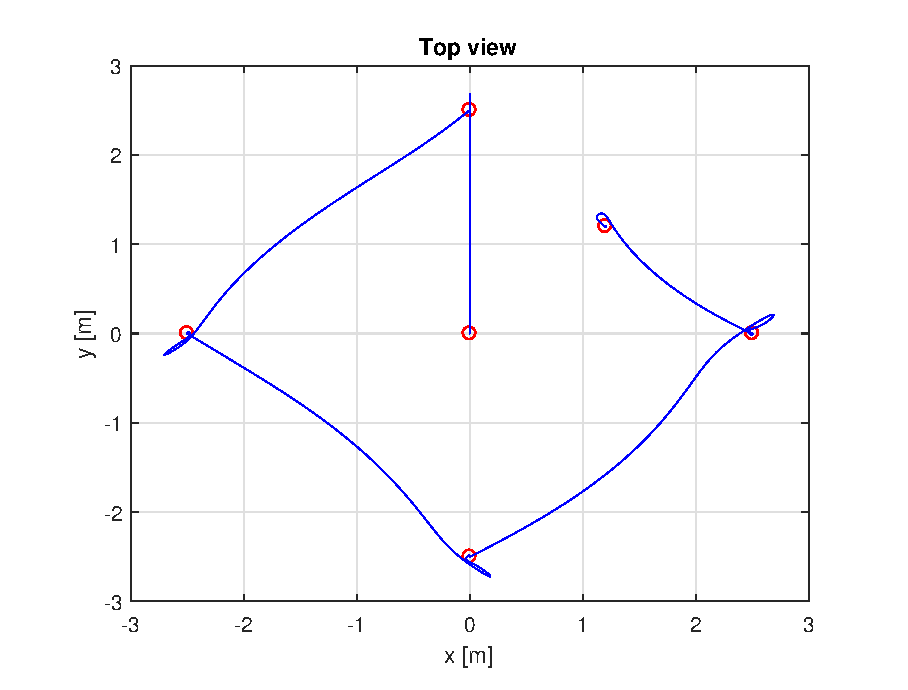
\includegraphics[width=\textwidth]{./LQR_load/Integrator/fig1.eps}
		\caption{top view}
	\end{subfigure}
	\begin{subfigure}[b]{0.3\textwidth}
		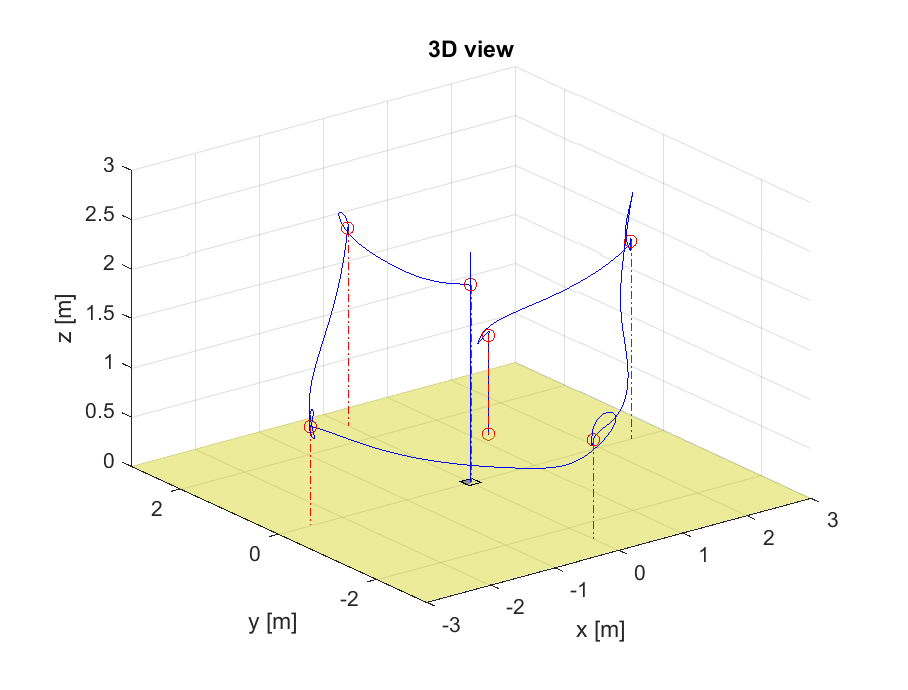
\includegraphics[width=\textwidth]{./LQR_load/Integrator/fig2.eps}
		\caption{3D view}
	\end{subfigure}
	\begin{subfigure}[b]{0.3\textwidth}
		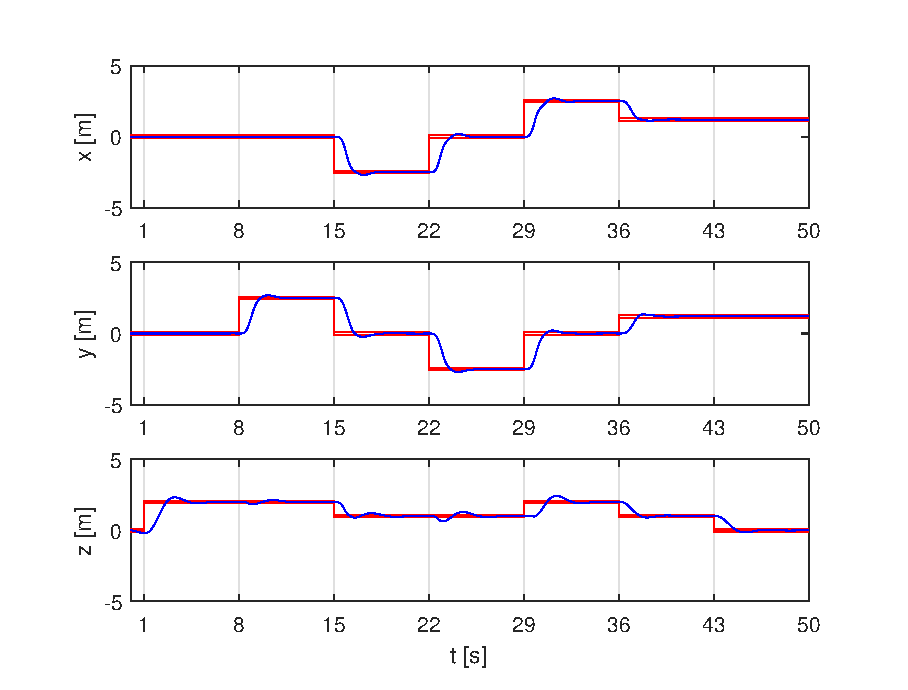
\includegraphics[width=\textwidth]{./LQR_load/Integrator/fig3.eps}
		\caption{individual axis}
	\end{subfigure}
	\begin{subfigure}[b]{0.3\textwidth}
		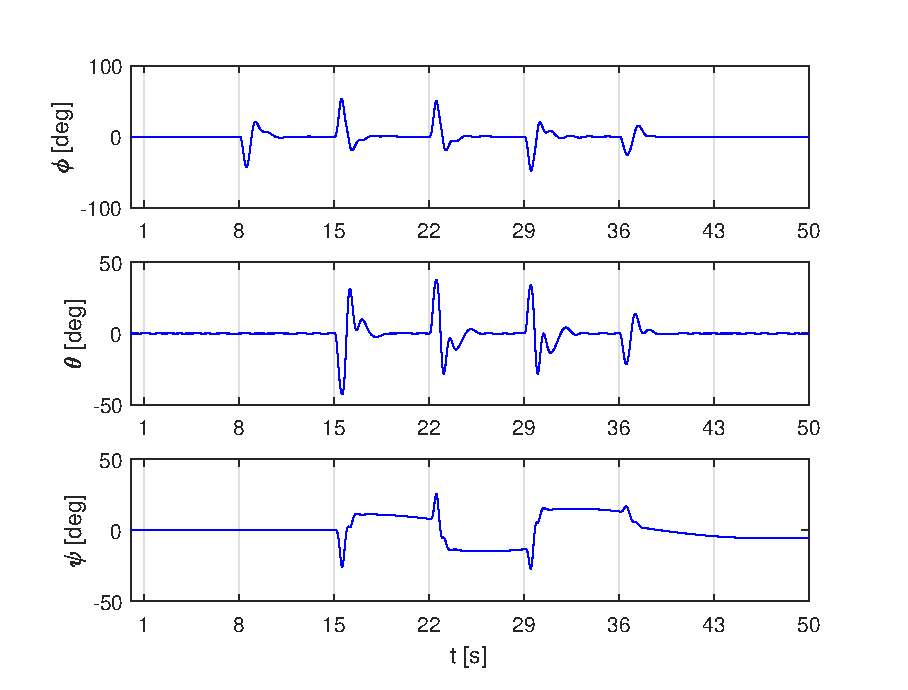
\includegraphics[width=\textwidth]{./LQR_load/Integrator/fig4.eps}
		\caption{angles}
	\end{subfigure}
	\begin{subfigure}[b]{0.3\textwidth}
		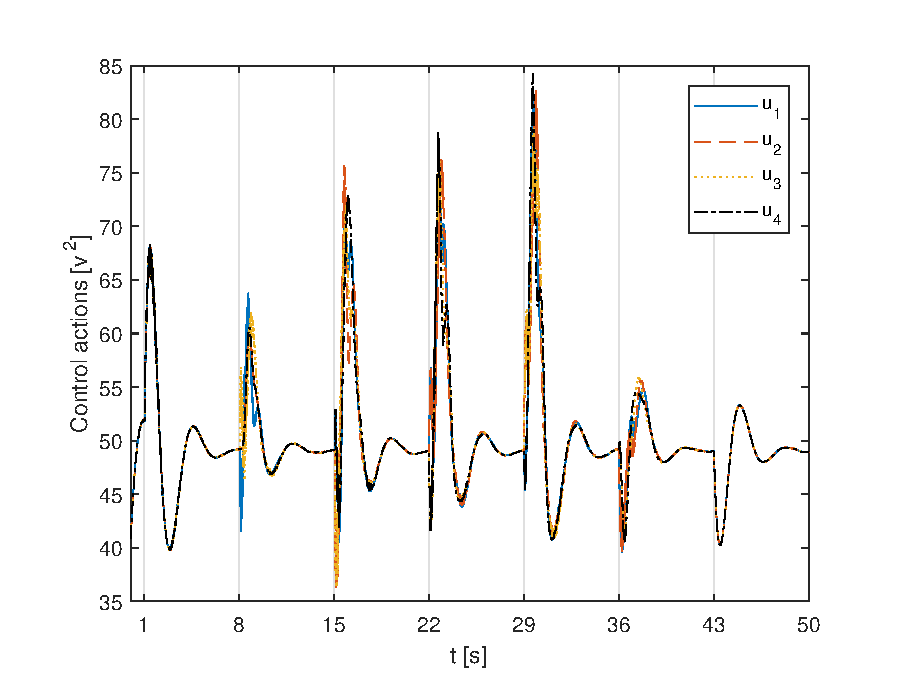
\includegraphics[width=\textwidth]{./LQR_load/Integrator/fig5.eps}
		\caption{actions}
	\end{subfigure}
	\caption{integrator with 0.1 load, average of 3.393 s}\label{fig:Integrator with load}
\end{figure}

\subsection{Fundamental difference integrator and full state-feedback controller}
The full-state feedback controller can only steer on the current situation. So when the x,y and z coordinates are different from the track it will compensate for this at a constant rate. It doesn't matter how long(so time, not distance) the copter is off the track it will keep compensating at this constant rate. 

The Integrator on the other hand will integrate the difference and so at first it will only compensate slightly but the longer the copter is off track the harder it will compensate. This is also part of the the reason why the integrator over compensates, and an additional weight must be set to the speeds $v_x$,$v_y$ and $v_z$.

The integrator is a discrete integrator with equal distance points, and equal weights to each value. If the Integrator has 20 high values then 3 low values will not significantly change the integration value. But 10 low values will significantly change the integration value. This integration is done at real time which means that the integration value is different if the situation changes. Which is the whole reason its more robust.

%The fundamental difference between the integral controller and the full state is that the integrator uses all of the past error values. As it integrates over all the errors. While the full state controller only looks at the current error. Obviously if you have more information you can control better, so the integrator has a distinct advantage over the full state controller.



% \appendix
% \section*{Codes}
% \addcontentsline{toc}{section}{Codes}
% \input{appendix/code.tex}

\end{document}
